\documentclass[tikz,border=10pt]{standalone}
\usepackage[T1]{fontenc}
\usepackage{lmodern}
\usepackage{xcolor}
\usetikzlibrary{arrows.meta}

\begin{document}
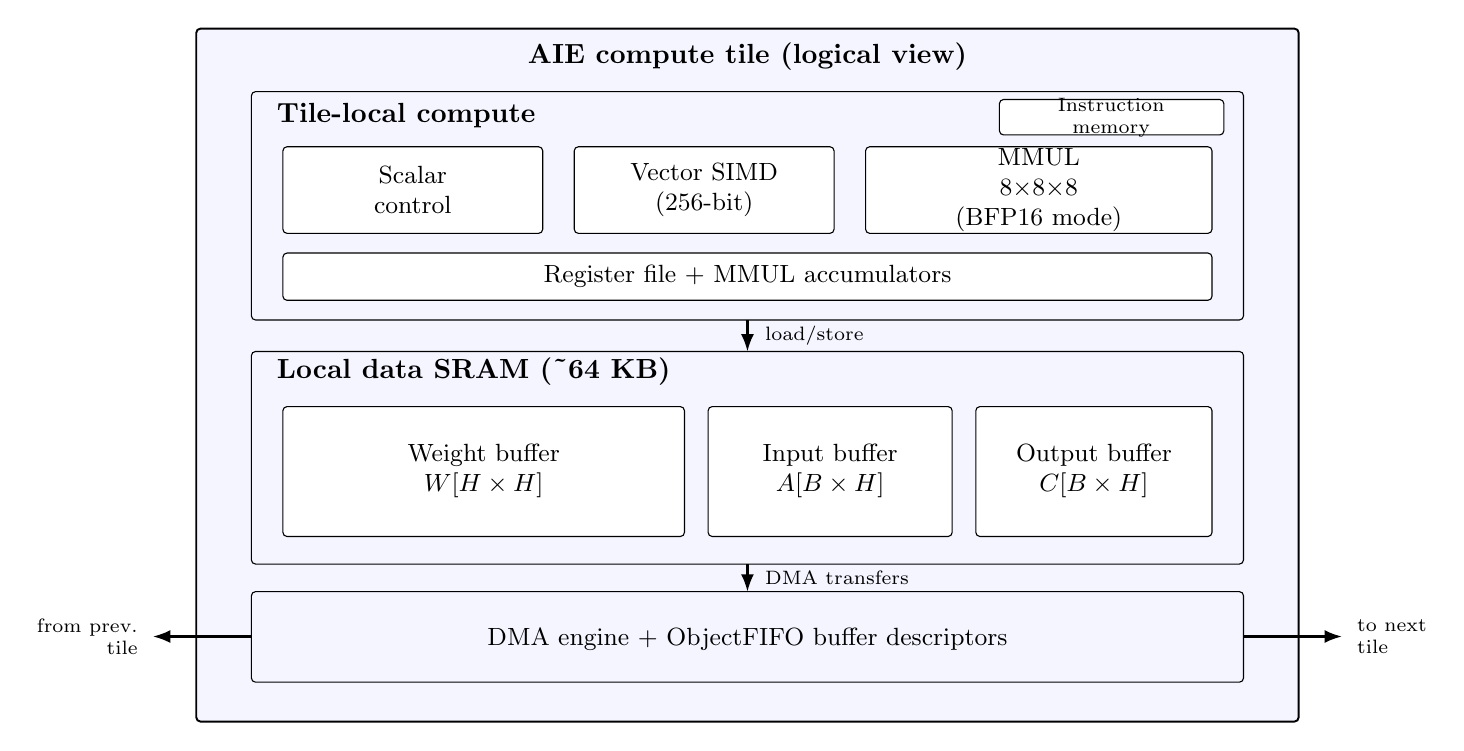
\begin{tikzpicture}[
  font=\small,
  >={Latex[length=2.2mm]},
  box/.style={draw, rounded corners=1.5pt, fill=blue!4},
  innerbox/.style={draw, rounded corners=1.5pt, fill=white},
  flow/.style={->, thick}
]
  \draw[box, line width=0.7pt] (0,0) rectangle (14,8.8);
  \node[font=\bfseries] at (7,8.45) {AIE compute tile (logical view)};

  \draw[box] (0.7,5.1) rectangle (13.3,8.0);
  \node[anchor=west, font=\bfseries] at (0.9,7.7) {Tile-local compute};
  \draw[innerbox] (1.1,6.2) rectangle (4.4,7.3);
  \draw[innerbox] (4.8,6.2) rectangle (8.1,7.3);
  \draw[innerbox] (8.5,6.2) rectangle (12.9,7.3);
  \node[align=center] at (2.75,6.75) {Scalar\\control};
  \node[align=center] at (6.45,6.75) {Vector SIMD\\(256-bit)};
  \node[align=center] at (10.7,6.75) {MMUL\\8$\times$8$\times$8\\(BFP16 mode)};
  \draw[innerbox] (1.1,5.35) rectangle (12.9,5.95);
  \node at (7.0,5.65) {Register file + MMUL accumulators};
  \draw[innerbox] (10.2,7.45) rectangle (13.05,7.9);
  \node[font=\scriptsize, align=center] at (11.62,7.67) {Instruction\\memory};

  \draw[box] (0.7,2.0) rectangle (13.3,4.7);
  \node[anchor=west, font=\bfseries] at (0.9,4.45) {Local data SRAM (\textasciitilde{}64 KB)};
  \draw[innerbox] (1.1,2.35) rectangle (6.2,4.0);
  \draw[innerbox] (6.5,2.35) rectangle (9.6,4.0);
  \draw[innerbox] (9.9,2.35) rectangle (12.9,4.0);
  \node[align=center] at (3.65,3.18) {Weight buffer\\$W[H\times H]$};
  \node[align=center] at (8.05,3.18) {Input buffer\\$A[B\times H]$};
  \node[align=center] at (11.4,3.18) {Output buffer\\$C[B\times H]$};

  \draw[box] (0.7,0.5) rectangle (13.3,1.65);
  \node at (7.0,1.05) {DMA engine + ObjectFIFO buffer descriptors};

  \draw[flow] (7.0,5.1) -- (7.0,4.7);
  \node[font=\scriptsize, anchor=west] at (7.1,4.9) {load/store};
  \draw[flow] (7.0,2.0) -- (7.0,1.65);
  \node[font=\scriptsize, anchor=west] at (7.1,1.82) {DMA transfers};

  \draw[flow] (0.7,1.08) -- (-0.55,1.08);
  \node[font=\scriptsize, anchor=east, align=right] at (-0.62,1.08) {from prev.\\tile};
  \draw[flow] (13.3,1.08) -- (14.55,1.08);
  \node[font=\scriptsize, anchor=west, align=left] at (14.62,1.08) {to next\\tile};
\end{tikzpicture}
\end{document}
